\documentclass[]{beamer}
%\documentclass[handout]{beamer}
\usetheme{Boadilla} 
%\usecolortheme{seagull}
%\setbeamerfont*{frametitle}{size=\normalsize,series=\bfseries}
%\setbeamertemplate{blocks}[default]%[shadow=false]

\setbeamertemplate{footnote}{\tiny\makebox[1em][l]{\insertfootnotemark}\insertfootnotetext\par}



%\setbeamertemplate{footnote}{\hangpara{1em}{1}\makebox[1em][l]{\insertfootnotemark}\scriptsize\insertfootnotetext\par}

%\definecolor{icml_tutorial}{RGB}{181,74,16}

%\setbeamercolor{title}{bg=icml_tutorial,fg=white}

%\usetheme{Boadilla}
\usefonttheme{professionalfonts}
%%\usecolortheme{seagull}
\usefonttheme[onlymath]{serif}
%
\setbeamertemplate{blocks}[rounded][shadow=false]

\usepackage{array}
%\usepackage{algorithm}
%\usepackage{algorithmic}
%\usepackage[english]{babel}
\usepackage{booktabs} 
\usepackage{graphicx}
\usepackage{amssymb}
\usepackage{amsmath}
\usepackage{stmaryrd} 
\usepackage{dsfont}
\usepackage{color,colortbl} 
\usepackage{pgfplots}
%\usepackage{bibentry}
\usepackage{algorithm}
\usepackage[noend]{algpseudocode}
\usepackage{tikz}
\usetikzlibrary{mindmap,trees}
\usetikzlibrary{decorations.pathreplacing}
\usetikzlibrary{decorations.pathmorphing}
\usetikzlibrary{arrows}
\usetikzlibrary{positioning}
\usetikzlibrary{decorations.text}
\usetikzlibrary{decorations.markings}
\usetikzlibrary{decorations.shapes}
\usetikzlibrary{shapes,snakes}
\usetikzlibrary{calc,trees,positioning,arrows,chains,shapes.geometric,
  decorations.pathreplacing,decorations.pathmorphing,shapes,matrix,shapes.symbols}
\usetikzlibrary{shapes.misc}

\usepackage{multirow}
% \usepackage{beamerthemesplit} // Activate for custom appearance



 
\newcommand{\lsize}{m}
\newcommand{\osize}{n}
\newcommand{\qsize}{q}
\newcommand{\odsize}{d}
\newcommand{\qdsize}{r}
\newcommand{\ispace}{\mathcal{X}}
\newcommand{\taskspace}{\mathcal{T}}
\newcommand{\objspace}{\mathcal{D}}
\newcommand{\anyspace}{\mathcal{X}}
\newcommand{\hypspace}{\mathcal{H}}
\newcommand{\kernelf}{k}
\newcommand{\gkernelf}{g}
\newcommand{\kkernelf}{\Gamma}
\newcommand{\dkernelm}{\bm{K}}
\newcommand{\tkernelm}{\bm{G}}
\newcommand{\kkernelm}{\bm{\Gamma}}
\newcommand{\regparam}{\lambda}
\newcommand{\idmatrix}{\bm{I}}
\newcommand{\trace}{\textnormal{tr}}
%\newcommand{\transpose}{^\textnormal{T}}
\newcommand{\transpose}{^\intercal}
\newcommand{\bm}[1]{\mathbf{#1}}
\newcommand{\ve}{\textnormal{vec}}
\newcommand{\mat}{\textnormal{mat}}
\newcommand{\diagv}{\textnormal{diag}_v}
\newcommand{\diagm}{\textnormal{diag}_m}
\newcommand{\LOO}{\text{LOO}}
\newcommand{\predfun}{f}
\newcommand{\filterfun}{\varphi}
\newcommand{\objset}{D}
\newcommand{\taskset}{T}
\newcommand{\labelvec}{\bm{y}}
\newcommand{\Algo}[1]{{#1}}


\setbeamertemplate{footline}[frame number]
\beamertemplatenavigationsymbolsempty 
%\logo{\includegraphics[height=1.2cm]{Figures/Kermit}}



\renewcommand{\Pr}{P}
\newcommand{\cumPr}{\mathbf{P}}
\renewcommand{\vec}[1]{\boldsymbol{#1}}
\newcommand{\brY}{\vec{Y}}
\newcommand{\given}{\, | \,}
\newcommand{\cumprob}{P}
\newcommand{\cumprobx}{P_{\vec{x}}}
\newcommand{\probx}{p_{\vec{x}}}
\newcommand{\probxi}[1]{p_{\vec{x}}^{(#1)}}
\newcommand{\invmarg}[1]{P_{\vec{x},#1}^{-1}}
\newcommand{\cop}{C}
\newcommand{\dcop}{c}
\newcommand{\copx}{C_{\vec{x}}}
\newcommand{\dcopx}{c_{\vec{x}}}
\newcommand{\mx}[1]{\mathbf{\mathrm{#1}}}
\newcommand{\maxprobxi}[1]{p_{\vec{x},max}^{(#1)}}
\newcommand{\minprobxi}[1]{p_{\vec{x},min}^{(#1)}}
\DeclareMathOperator*{\argmax}{\arg \max}
\DeclareMathOperator*{\argmin}{\arg \min}

\newcommand{\Fb}{F}
\newcommand{\loss}{L}
\newcommand{\ells}{\tilde{\ell}}
\newcommand{\regret}{\textnormal{Reg}}
\newcommand{\lossrank}{L_{\textnormal{\scriptsize{rnk}}}}
\newcommand{\ellrank}{\ell_{\textnormal{\scriptsize{rnk}}}}
\newcommand{\regretrank}{{\textnormal{Reg}}_{\textnormal{\scriptsize{rnk}}}}
%\newcommand{\lossranktilde}{L_{\widetilde{rnk}}}
%\newcommand{\regretranktilde}{{\textnormal{Reg}}_{\widetilde{rnk}}}
\newcommand{\lossranktilde}{\lossrank}
\newcommand{\regretranktilde}{\regretrank}
\newcommand{\lossexp}{L_{\textnormal{\scriptsize{exp}}}}
\newcommand{\ellexp}{\ells_{\textnormal{\scriptsize{exp}}}}
\newcommand{\regretexp}{{\textnormal{Reg}}_{\textnormal{\scriptsize{exp}}}}
\newcommand{\losslog}{L_{\textnormal{\scriptsize{log}}}}
\newcommand{\elllog}{\ells_{\textnormal{\scriptsize{log}}}}
\newcommand{\regretlog}{{\textnormal{Reg}}_{\textnormal{\scriptsize{log}}}}
\newcommand{\lossrankbar}{L_{\textnormal{\scriptsize{br}}}}
\newcommand{\ellrankbar}{\ell_{\textnormal{\scriptsize{br}}}}
\newcommand{\regretrankbar}{{\textnormal{Reg}}_{\textnormal{\scriptsize{br}}}}

\newcommand{\sgn}[1]{\textrm{sgn}\left(#1\right)}
%\newcommand{\bm}{\mathds{1}}
\newcommand{\ZO}{0/1 }
\newcommand{\bx}{\boldsymbol{x}}
\newcommand{\by}{\boldsymbol{y}}
\newcommand{\bh}{\boldsymbol{h}}
\newcommand{\bY}{\boldsymbol{Y}}
\newcommand{\bX}{\boldsymbol{X}}
\newcommand{\bz}{\boldsymbol{z}}
%\newcommand{\bm}{\mathds{1}}
\newcommand{\assert}[1]{\llbracket #1 \rrbracket}
%\newcommand{\assert}[1]{\bm [ #1 ] } %[\llbracket #1 \rrbracket}
\newcommand{\colorcell}{\multicolumn{1}{>{\columncolor{DarkGreen}}l}{}}
\newcommand{\graytextcell}[1]{\begin{color}{gray}#1\end{color}}
\newcommand{\calX}{\mathcal{X}}
\newcommand{\calY}{\mathcal{Y}}
\newcommand{\calH}{\mathcal{H}}
\newcommand{\calL}{\mathcal{L}}
\newcommand{\calO}{\mathcal{O}} 
\newcommand{\calC}{\mathcal{C}} 

%\newcommand{\loss}{L}
%\newcommand{\regret}{\textnormal{Reg}}
\newcommand{\lossell}{L_{\ell}}
\newcommand{\regretell}{\textnormal{Reg}_{\ell}}
%\newcommand{\lossrank}{L_{\textnormal{\scriptsize{rank}}}}
%\newcommand{\regretrank}{{\textnormal{Reg}}_{\textnormal{\scriptsize{rank}}}}
%\newcommand{\sgn}[1]{\textrm{sgn}\left(#1\right)}
%\newcommand{\bm}{\mathds{1}}

\definecolor{putblue}{RGB}{0,0,124}
\definecolor{putred}{RGB}{204,33,69}
\renewcommand{\alert}[1]{\textbf{\color{putblue} #1}}
\renewcommand{\emph}[1]{\textbf{\color{putblue}#1}}
%\renewcommand{\emph}[1]{\textbf{\color{icml_tutorial}#1}}


\setbeamercolor{title}{bg=white,fg=putblue}
\setbeamercolor{subtitle}{bg=white,fg=putblue}

%\newcommand {\autographics}[1] {
  %\begin{center}
    %\includegraphics[width=\textwidth,height=0.85\textheight,keepaspectratio]{#1}
  %\end{center}
%}
%\newcommand {\autographicswithsize}[2] {
  %\begin{center}
    %\includegraphics[width=\textwidth,height=#2\textheight,keepaspectratio]{#1} 
  %\end{center}
%}

%\newcommand {\autographicswithsizew}[2] {
  %\begin{center}
  %\vskip-20pt
    %\includegraphics[width=\textwidth,width=#2\textheight,keepaspectratio]{#1}
  %\vskip5pt
  %\end{center}
%}

%\def\newblock{\hskip .11em } %plus .33em minus .07em}


\title[]{Multi-Target Prediction:\\ 
A Unifying View on Problems and Methods}
\author[Willem Waegeman]{Willem Waegeman} 
%\author[Eyke]{Eyke H\"ullermeier}
%\date[NIPS 2015]{NIPS: extreme classification workshop\\December 12, 2015}
\institute[VFU] % (optional)
{
  \inst{}
Department of Data Analysis and Mathematical Modelling, Ghent University, Belgium \\
}

\date{September 30th 2019 }

\begin{document}

\frame{\titlepage}

\section{Introduction}

%\begin{frame}[plain]
        %\begin{tikzpicture}[remember picture,overlay]
            %\node[at=(current page.center)] {
                %\includegraphics[scale=0.35]{pics/flanders}
            %};
        %\end{tikzpicture}
     %\end{frame}
		
		\begin{frame}[plain]
        \begin{tikzpicture}[remember picture,overlay]
            \node[at=(current page.center)] {
                \includegraphics[scale=0.17]{Figures/and}
            };
        \end{tikzpicture}
     \end{frame}

%\section{Introduction}

\begin{frame}{Multi-label classification: \\
the example of document categorization}
% voorbeeldje met boeken
\includegraphics[width=0.9\textwidth,trim = 0 0 100 100,clip]{Figures/pictures/Slide2}
\end{frame}

\begin{frame}[plain]
        \begin{tikzpicture}[remember picture,overlay]
            \node[at=(current page.center)] {
                \includegraphics[width=0.7\textwidth]{pics/proteinl}
            };
        \end{tikzpicture}
     \end{frame}

\begin{frame}{Multivariate regression: \\
the example of protein-ligand interaction prediction}
% voorbeeldje met boeken
\includegraphics[width=0.9\textwidth,trim = 0 0 100 100,clip]{Figures/pictures/Slide1}
\end{frame}

\begin{frame}[plain]
        \begin{tikzpicture}[remember picture,overlay]
            \node[at=(current page.center)] {
                \includegraphics[width=\textwidth]{Figures/school_shopping}
            };
        \end{tikzpicture}
     \end{frame}

\begin{frame}{Multi-task learning: \\
the example of predicting student marks}
% voorbeeldje met boeken
\includegraphics[width=0.9\textwidth,trim = 0 0 100 100,clip]{Figures/pictures/Slide3}
\end{frame}



%\begin{frame}{Other cool applications: ecology}
   %\center 
   %\includegraphics[width=10cm]{Figures/foodweb.jpg}
   %\vfill
   %%Predicting links between \alert{people}
 %% social network prediction, protein ligand prediction, food pairing, image analysis: voorbeeld?
%\end{frame}

%\begin{frame}{Other cool applications: food pairing}
   %\center 
   %\includegraphics[width=\textwidth]{Figures/ingredients}
   %\vfill
 %% social network prediction, protein ligand prediction, food pairing, image analysis: voorbeeld?
%\end{frame}

%
%\begin{frame}{The two-step ridge regression}
%Prediction function:
%
%$$
%f(d, t) = \boldsymbol{\phi}(d)^\intercal\mathbf{W}  \boldsymbol{\psi}  (t) 
%$$
%
%Parameters can be found by solving:
%$$
%\boldsymbol{\Phi}^\intercal\mathbf{Y}\boldsymbol{\Psi} = (\boldsymbol{\Phi}^\intercal\boldsymbol{\Phi}+\lambda_d\mathbf{I})\mathbf{W}(\boldsymbol{\Psi}^\intercal\boldsymbol{\Psi}+\lambda_t\mathbf{I})
%$$
%\pause
%Two hyperparameters: $\lambda_d$ and $\lambda_t$!
%\end{frame}

\begin{frame}{There are a lot of multi-target prediction problems around...}

\begin{center}
\includegraphics[width=\textwidth,trim = 0 0 0 70,clip]{Figures/pictures/Slide20}
\end{center}

\end{frame}

\begin{frame}{Accompanying article}

\begin{center}
\includegraphics[width=\textwidth,trim = 0 0 0 0,clip]{Figures/dami}\\
Data Mining and Knowledge discovery, 2019. 
\end{center}

\end{frame}


%%% begin changes %%%


\section{A unifying view on MTP problems}


\begin{frame}{Overview of this talk}

\tableofcontents

\end{frame}




%\begin{frame}
%\frametitle{Multi-target prediction}
%\begin{itemize}
%\item \emph{Multi-Target Prediction:} For a feature vector $\bx$ predict accurately \\a vector of responses $\by$ using a function $\bh(\bx)$:
%$$
%\bx = (x_1,x_2,\ldots,x_p) \xrightarrow{~~\bh(\bx)~~} \by = (y_1, y_2, \ldots, y_m)
%$$
%\item \emph{Main challenges:} 
%\begin{itemize}
%\item Appropriate modeling of target dependencies between targets 
%$$
%y_1, y_2, \ldots, y_m
%$$
%\item A multitude of multivariate loss functions defined over the output vector 
%$$\ell(\by, \bh(\bx))$$
%%to measure the quality of prediction.
%\end{itemize}
%\item \emph{Main question:} %Can we improve over independent models trained for each target?
%\begin{itemize}
%\item Can we improve over independent models trained for each target? 
%\end{itemize}
%\item \emph{Two views:} %the individual target and joint target view.
%\begin{itemize}
%\item The individual-target view
%\item The joint-target view
%\end{itemize}
%\end{itemize}
%
%\end{frame}

%\begin{frame}{General framework}
%\begin{definition}
%A multi-target prediction setting is characterized by instances $\vec{x} \in \mathcal{X}$ and targets $\vec{t} \in \mathcal{T}$ with the following properties: 
%\begin{itemize} 
%\item[1.] A training dataset consists of triplets $(\vec{x}_i,\vec{t}_j,y_{ij})$, where $y_{ij} \in \mathcal{Y}$.  
%\item[2.] In total $n$ instances and $m$ targets are observed during training, with $n$ and $m$ finite numbers. 
%\item[3.]As such, the scores $y_{ij}$ of the training data can be arranged in an $n \times m$ matrix $Y$.
%\item[4.] The score set $\mathcal{Y}$ is one-dimensional. It consists of nominal, ordinal or real values.  
%\item[5.] The goal consists of making predictions for any instance-target couple $(\vec{x},\vec{t}) \in \mathcal{X} \times \mathcal{T}$.   
%\end{itemize}
%\end{definition}
%\end{frame}


%
%\begin{frame}{Multivariate regression}
%% voorbeeldje met boeken
%\includegraphics[width=0.9\textwidth,trim = 0 0 100 100,clip]{Figures/pictures/Slide1}
%\end{frame}
%
%
%\begin{frame}{Conventional MTP settings}
%\begin{definition}[Multi-task learning] 
%A multi-task learning problem is a specific instantiation of the general framework, which exhibits the following additional properties: 
%\begin{enumerate}
%\item[P5.] The cardinality of $\mathcal{T}$ is $m$; this implies that all targets are observed during training. 
%\item[P6.] No side information is available for targets. Again, the target space can hence be taken as $\mathcal{T} = \{1,...,m\}$.   
%\item[P8a.] The score set is homogenous across columns of $Y$, e.g., $\mathcal{Y} = \{0,1\}$ or $\mathcal{Y} = \mathbb{R}$.
%\end{enumerate}
%\end{definition}
%\end{frame}
%
%
%\begin{frame}{Multi-task learning}
%% voorbeeldje met boeken
%\includegraphics[width=0.9\textwidth,trim = 0 0 100 100,clip]{Figures/pictures/Slide3}
%\end{frame}
%
%
%\begin{frame}{Conventional MTP settings}
%\begin{definition}[Multi-label classification] 
%A multi-label classification problem is a specific instantiation of the general framework, which exhibits the following additional properties: 
%\begin{enumerate}
%\item[P5.] The cardinality of $\mathcal{T}$ is $m$; this implies that all targets are observed during training. 
%\item[P6.] No side information is available for targets. Again, without loss of generality, we can hence identify targets with natural numbers, such that the target space is $\mathcal{T} = \{1,...,m\}$. 
%\item[P7.] The score matrix $Y$ has no missing values. 
%\item[P8b.] The score set is $\mathcal{Y} = \{0,1\}$. 
%\end{enumerate}
%\end{definition}
%\end{frame}
%
%\begin{frame}{Multi-label classification}
%% voorbeeldje met boeken
%\includegraphics[width=0.9\textwidth,trim = 0 0 100 100,clip]{Figures/pictures/Slide2}
%\end{frame}
%
%
%\begin{frame}{Conventional MTP settings}
%\begin{definition}[Label ranking] 
%A multi-label classification problem is a specific instantiation of the general framework, which exhibits the following additional properties: 
%\begin{enumerate}
%\item[P5.] The cardinality of $\mathcal{T}$ is $m$; this implies that all targets are observed during training. 
%\item[P6.] No side information is available for targets. Again, without loss of generality, we can hence identify targets with natural numbers, such that the target space is $\mathcal{T} = \{1,...,m\}$. 
%\item[P7.] The score matrix $Y$ has no missing values. 
%\item[P8c.] The score set is $\mathcal{Y} = \{1, \ldots , m\}$, and the scores (interpreted as ranks) are such that $y_{ij} \neq y_{ik}$ for all $1 \leq j,k \neq m$. 
%\end{enumerate}
%\end{definition}
%\end{frame}
%
%
%
%
%
%\begin{frame}{Conventional MTP settings}
%\begin{itemize}
%\item
%In \emph{label ranking}\footnote{E.H., J.\ F\"urnkranz, W.\ Cheng, K.\ Brinker. Label Ranking by Learning Pairwise Preferences, Artificial Intelligence, 172, 2008.}, each instance is associated with a ranking (total order) of the targets.
%\end{itemize}
%%\vspace{0.8cm}
%\begin{center}
%\includegraphics[width=0.8\textwidth]{Figures/pictures/labelranking}
%\end{center}
%\end{frame}
%




\begin{frame}{Let's assume a document hierarchy: \\
How would you call this machine learning problem?}
\begin{center}
\includegraphics[width=0.75\textwidth,trim = 0 0 100 0,clip]{Figures/pictures/Slide5}
\end{center}
\end{frame}

\begin{frame}{Let's assume a target representation: \\
How would you call this machine learning problem?}
\begin{center}
\includegraphics[width=0.8\textwidth,trim = 0 0 100 30,clip]{Figures/pictures/Slide6}
\end{center}

\end{frame}

\begin{frame}{Let's assume a target representation: \\
How would you call this machine learning problem?}
\vspace{0.8cm}
\includegraphics[width=0.9\textwidth,trim = 0 0 0 90,clip]{Figures/pictures/Slide4}

\end{frame}




%
%\begin{frame}{Learning with side information on targets}
%\begin{itemize}
%\item Additional side information about the target space is available.
%\item Examples: 
%\begin{itemize}
%\item Representation for the target molecules in drug design application (\emph{structured representation}).
%\item Taxonomy on document categories (\emph{hierarchy}).
%\item Information about schools and courses (geographical location, qualifications of the teachers, reputation of the school, etc.) in student mark forecasting application (\emph{feature representation}).
%\end{itemize}
%\item Such problems are often referred to as dyadic prediction, link prediction, or network inference settings.
%\end{itemize}
%\end{frame}
%
%
%\begin{frame}{Learning with side information on targets}
%\begin{itemize}
%\item
%Generally speaking, such settings cover problems that obey the four properties listed in the MTP definition. 
%\item Labels $y_{ij}$ can be arranged in a matrix $Y$, which is often sparse. 
%\item Thus, one may argue that \emph{dyadic prediction} is nothing else than \emph{multi-task learning with task features}. 
%\item However, MTP terminology is rarely used in the dyadic prediction literature. 
%\end{itemize}
%\end{frame}
%
%
%
%
%
%\begin{frame}{Inductive versus transductive learning problems}
%\begin{itemize} 
%\item In the previous problems, 
%\begin{itemize}
%\item predictions need be be generated for novel instances, 
%\item whereas the set of targets is known beforehand and observed during the training phase.
%\end{itemize}
%\item These problems are \emph{inductive} w.r.t.\ instances and \emph{transductive} w.r.t.\ targets.
%\item   
%\emph{Side information} is of crucial importance for generalizing to novel targets that are unobserved during the training phase.
%%such as a novel target molecule in the drug design example, a novel tag in the document annotation example, or a novel course in the student grading example. 
%\end{itemize}
%\end{frame}
%

\begin{frame}{Inductive versus transductive learning problems}
% voorbeeldje met boeken
%\vspace{0.6cm}
$$\qquad g(.,.): \mbox{target similarity}$$

\includegraphics[width=0.9\textwidth,trim = 0 0 0 60,clip]{Figures/pictures/Slide7}
\end{frame}

\begin{frame}{Important subdivision of different learning settings}
   \center
	\vspace{0.4cm}
   \includegraphics[width=0.9\textwidth]{Figures/pictures/Slide16} % requires the graphicx package
\end{frame}


\begin{frame}{General framework}
\begin{definition}[Multi-target prediction]
A multi-target prediction setting is characterized by instances $\vec{x} \in \mathcal{X}$ and targets $\vec{t} \in \mathcal{T}$ with the following properties: 
\begin{itemize} 
\item[P1.] A training dataset $\mathcal{D}$ consists of triplets $(\vec{x}_i,\vec{t}_j,y_{ij})$, where $y_{ij} \in \mathcal{Y}$ denotes a score that characterizes the relationship between the instance $\vec{x}_i$ and the target $\vec{t}_j$.  
\item[P2.] In total, $n$ different instances and $m$ different targets are observed during training, with $n$ and $m$ finite numbers. Thus, the scores $y_{ij}$ of the training data can be arranged in an $n \times m$ matrix $Y$, which is in general incomplete, i.e., $Y$ has missing values.
\item[P3.] The score set $\mathcal{Y}$ is one-dimensional. It consists of nominal, ordinal or real values.  
\item[P4.] The goal consists of predicting scores for any instance-target couple $(\vec{x},\vec{t}) \in \mathcal{X} \times \mathcal{T}$.   
\end{itemize}
\end{definition}

\end{frame}




\begin{frame}{Specific MTP settings: one example}
\begin{definition}[Multivariate regression] 
A multivariate regression problem is a specific instantiation of the general framework, which exhibits the following additional properties: 
\begin{enumerate}
\item[P5.] The cardinality of $\mathcal{T}$ is $m$. This implies that all targets are observed during training. 
\item[P6.] No side information is available for targets. Without loss of generality, we can hence assign the numbers $1$ to $m$ as identifiers to targets, such that the target space is $\mathcal{T} = \{1,...,m\}$. 
\item[P7.] The score matrix $Y$ has no missing values. 
\item[P8.] The score set is $\mathcal{Y} = \mathbb{R}$. 
\end{enumerate}
\end{definition}
\end{frame}



\section{A unifying view on MTP methods}


\begin{frame}{Overview of this talk}

\tableofcontents

\end{frame}

\begin{frame}{A unifying view on MTP methods}

\begin{center}
\includegraphics[scale=0.3]{pics/tools}

\begin{tabular}{ll}
\hline
Group of methods & Applicable setting \\
\hline
\hline
\alert{Independent models} & B \\
Similarity-enforcing methods & B   \\ 
Relation-exploiting methods & B and D  \\
Relation-constructing methods & B \\
Representation-exploiting methods & B and D \\
Representation-constructing methods & A and B \\
\hline  
\end{tabular}
\end{center}
\end{frame}

%\begin{frame}{Different learning settings revisited}
   %\center
	%\vspace{0.4cm}
   %\includegraphics[width=0.9\textwidth]{Figures/pictures/Slide16} % requires the graphicx package
%\end{frame}


\begin{frame}{A baseline method:\\
learning a model for each target independently}
% voorbeeldje met boeken
\includegraphics[width=0.9\textwidth,trim = 0 0 100 100,clip]{Figures/pictures/Slide13}
\end{frame}

\begin{frame}{A baseline method:\\
learning a model for each target independently}
% voorbeeldje met boeken
\includegraphics[width=0.9\textwidth,trim = 0 0 100 100,clip]{Figures/pictures/Slide14}
\end{frame}

\begin{frame}{A baseline: Independent Models}
% voorbeeldje met boeken
\includegraphics[width=0.9\textwidth,trim = 0 0 100 100,clip]{Figures/pictures/Slide15}
\end{frame}

\begin{frame}{A baseline: Independent Models}
% voorbeeldje met boeken
\vspace{0.5cm}
Linear basis function model for $i$-th target: 
\begin{equation*}
f_i(\vec{x}) = \vec{a}_i^\intercal \phi(\vec{x}) \,,
\label{eq:binrel}
\end{equation*}
Solving as a joint optimization problem: 
\begin{equation*}
\label{eq:multiridge}
\min_A ||Y - XA ||^2_F +  \sum_{i=1}^m \lambda_i \,||\vec{a}_i||^2 \,,
\end{equation*}
$$Y: (n \times m) \qquad  X: (n \times p) \qquad A: (p \times m)$$
With the following notations: 
\begin{equation*}
\label{eq:notation}
X = \begin{bmatrix} \phi(\vec{x}_1)^T \\ \vdots \\ \phi(\vec{x}_n)^T \end{bmatrix} \qquad A = [\vec{a}_1 \quad \cdots \quad \vec{a}_m] \,.
\end{equation*}
%Hamming loss as alternative for binary labels: 
%$${\displaystyle L_{\textit{Ham}}(\vec{y},\hat{\vec{y}}) = \sum_{j=1}^m I(y_j = \hat{y}_j)}$$


\end{frame}
%
%\begin{frame}{The results section of a typical MTP paper...}
%\begin{center}
%\includegraphics[scale=0.45, trim = 0 50 0 100,clip]{Figures/barplots} \\
%
%Independent models a.k.a.\ binary relevance, models that do not exploit target dependencies, one-versus-all, etc.
%\end{center}
%\end{frame}
%
%
%\begin{frame}
%
%\begin{center}
%Learning a model for each target independently is still state-of-the-art in extreme multi-label classification\footnote{Babbar and Sch\"olkopf, DISMEC: Distributed Sparse Machines for Extreme Multi-label classification, WSDM 2017}:
%
%\includegraphics[scale=0.3]{Figures/dismec} 
%\end{center}
%
%\end{frame}

%%%%%%%%%%%%%%%%%%%%%%%%%%%%%%%%%%%%%%%%%%%%%%%%%%%%%%%%%%%%%%%%%%%%%%%%%%%%%% 
%%%%%%%%%%%%%%%%%%%%%%%%%%%%%%%%%%%%%%%%%%%%%%%%%%%%%%%%%%%%%%%%%%%%%%%%%%%%%% 

%%%%%%%%%%%%%%%%%%%%%%%%%%%%%%%%%%%%%%%%%%%%%%%%%%%%%%%%%%%%%%%%%%%%%%%%%%%%%% 
%%%%%%%%%%%%%%%%%%%%%%%%%%%%%%%%%%%%%%%%%%%%%%%%%%%%%%%%%%%%%%%%%%%%%%%%%%%%%% 
%\frame{
  %\frametitle{ DiSMEC - Distributed Sparse Machines for XMC }
%
%\begin{algorithmic}[1]
 %\Require  {Training data $\mathcal{T} = \{(\vec{x}_1,\vec{y}_1) \ldots (\vec{x}_n,\vec{y}_n) \}$, input dimensionality $p$, label set $\{1 \ldots m\}$, $B=\lfloor\frac{m}{1000}\rfloor+1$  and pruning threshold $\Delta$}
%
%\Ensure{Learnt $p \times m$ matrix $A$ in sparse format} \pause 
%
%\State Load single copy of input vectors $X = \{\vec{x}_1 \ldots \vec{x}_n \}$ in the main memory  %\Comment{\textit{Refactor data without replication}} 
%
%\State Load binary sign vectors $\vec{s}_{j} = \{+1,-1\}_{i=1}^n$ separately for each label \pause 
%
%\For{$\{b=0; b < B; b++ \}$} \Comment{\alert{1st parallelization}}
%
        %\State \#pragma omp parallel for private($j$)  \Comment{\alert{2nd parallelization}}
%
       %\For{$\{j=b\times1000; j \leq (b + 1)\times1000; j++ \}$}
%
%\State Using $(\vec{X}, \vec{s}_{j})$, train weight vector $\vec{a}_{j}$ on a single core
%
%\State \alert{Prune ambiguous weights} in $\vec{a}_{j}$ 
%\EndFor
%
%\State \Return $p \times 1000$ matrix $A$  
%
%\EndFor
%
%\State \Return $p \times m$ weight matrix $A$ 
%\end{algorithmic} \pause 
%\begin{itemize} 
%\item Learns model for LSHTCWiki-325K in 6 hours on 400 cores
%\item Model size is 3GB due to pruning step
%\end{itemize}
%}
%
%\frame{
  %\frametitle{ Distribution of Learnt Weights}
%
%\begin{columns}
%\column{0.5\columnwidth}
%\begin{figure}[ht]
%\centering
%\includegraphics[width=\textwidth]{Figures/wiki10nonsparabs0p8.png}
%\caption{Before pruning}
%\end{figure}
%
%%\end{itemize}
%\column{0.5\columnwidth}
%\begin{figure}[ht]
%\centering
%\includegraphics[width=\textwidth]{Figures/l2c1abs0p8.png}
%\caption{After pruning small weights}
%\end{figure}
%\end{columns}
%\begin{itemize}
%\item Of the 3 Billion weights, 97\% are s.t, $A_ij \leq |0.01|$, and hence non-discriminative
%\item Storing them leads to large model sizes but no benefit in classification
%\end{itemize}
%
%}





\begin{frame}{A unifying view on MTP methods}

\begin{center}
\includegraphics[scale=0.3]{pics/tools}

\begin{tabular}{ll}
\hline
Group of methods & Applicable setting \\
\hline
\hline
Independent models & B \\
Similarity-enforcing methods & B   \\ 
Relation-exploiting methods & B and D  \\
Relation-constructing methods & B \\
\alert{Representation-exploiting methods} & B and D \\
Representation-constructing methods & A and B \\
\hline  
\end{tabular}
\end{center}
\end{frame}

\begin{frame}{Different learning settings revisited}
   \center
	\vspace{0.4cm}
   \includegraphics[width=0.9\textwidth]{Figures/pictures/Slide16} % requires the graphicx package
\end{frame}


%\begin{frame}{Different learning settings revisited}
   %\center
	%\vspace{0.4cm}
   %\includegraphics[width=0.9\textwidth]{Figures/pictures/Slide16} % requires the graphicx package
%\end{frame}
%
%\begin{frame}{An example revisited}
%\begin{center}
%\includegraphics[width=0.8\textwidth,trim = 0 0 100 30,clip]{Figures/pictures/Slide6}
%\end{center}
%
%\end{frame}

%\begin{frame}{Two examples revisited}
%\vspace{0.8cm}
%\includegraphics[width=0.9\textwidth,trim = 0 0 0 90,clip]{Figures/pictures/Slide4}
%
%\end{frame}

\begin{frame}{A target representation in computer vision}

\begin{center}
\includegraphics[scale=0.4]{Figures/semanticclasses} \\
Target representations are the key element of zero-shot learning methods\footnote{Examples taken from the CVPR 2016 Tutorial on Zero-shot learning for Computer Vision} 
\end{center}

\end{frame}

\begin{frame}{Target representations can take many forms}

\begin{center}
\includegraphics[width=\textwidth,trim = 0 0 0 90,clip]{Figures/representations}
\end{center}

\end{frame}

\begin{frame}{Learning target embeddings from text: Word2Vec}

Predict the probability of the next word $w_t$ given the previous words $h$\footnote{Mikolov et al., Efficient Estimation of Word Representations in
Vector Space, Arxiv 2013}:
$$P(w_t \given h) = \frac{\exp(f(w_t,h))}{\sum_{\mathrm{all words}} \exp(f(w_t,h))}$$
\begin{columns}
\begin{column}{5cm}
\includegraphics[scale=0.2]{Figures/word2vec}
\end{column}
\begin{column}{6cm}
\hspace{1cm} \includegraphics[scale=0.2]{Figures/kingqueen}
\end{column}
\end{columns}



\end{frame}


\begin{frame}{Kronecker kernel ridge regression}

\vspace{0.5cm}
Pairwise model representation in the primal: 
\begin{equation*}
\label{eq:pairwise}
f(\vec{x},\vec{t}) = \vec{w}^T \left(\phi(\vec{x}) \otimes \psi(\vec{t}) \right) 
\end{equation*}
Kronecker product pairwise kernel in the dual\footnote{Stock et al., A comparative study of pairwise learning methods based on kernel ridge regression, Neural Computation 2018}:
\begin{eqnarray*} 
f(\vec{x},\vec{t})= \sum_{(\bar{\vec{x}},\bar{\vec{t}}) \in \mathcal{D}} \alpha_{(\bar{\vec{x}},\bar{\vec{t}})}  k(\vec{x},\bar{\vec{x}}) \cdot g(\vec{t},\bar{\vec{t}})  = \sum_{(\bar{\vec{x}},\bar{\vec{t}}) \in \mathcal{D}} \alpha_{(\bar{\vec{x}},\bar{\vec{t}})} \Gamma((\vec{x},\vec{t}),(\bar{\vec{x}},\bar{\vec{t}})) 
\end{eqnarray*}
Least-squares minimization with 
$\bm{z} = \textrm{vec}{(Y)}$: 
$$ \min_{\bm{\boldsymbol\alpha}} \, ||\bm{\kkernelm}\bm{\boldsymbol\alpha} -\bm{z} ||^2_2 +\regparam\bm{\boldsymbol\alpha }\transpose\kkernelm\bm{\boldsymbol\alpha} $$


\end{frame}

%
%\begin{frame}{Two-step zero-shot learning\footnote{Pahikkala et al. A two-step approach for solving full and almost full cold-start problems in dyadic prediction, ECML/PKDD 2014.} \footnote{Romero-Paredes and Torr, An embarrassingly simple approach to zero-shot learning, ICML 2015.}}
%\begin{columns}[c]
%\column{0.6\textwidth}
  %\center 
   %\includegraphics[width=0.7\textheight]{Figures/concept2SRLS}
%
%\column{0.4\textwidth}
%\begin{enumerate}
%\item Build a kernel ridge regression model to generalize to \alert{new instances}
%\item Build a kernel ridge regression model to generalize to \alert{new tasks}
%\end{enumerate}
%\end{columns}
%\end{frame}

\begin{frame}{Two-step zero-shot learning\footnote{Pahikkala et al. A two-step approach for solving full and almost full cold-start problems in dyadic prediction, ECML/PKDD 2014.} \footnote{Romero-Paredes and Torr, An embarrassingly simple approach to zero-shot learning, ICML 2015.}}
% voorbeeldje met boeken
\vspace{0.5cm}
\includegraphics[width=0.75\textwidth,trim = 0 0 0 90,clip]{Figures/pictures/Slide8}
\end{frame}


\begin{frame}{Two-step zero-shot learning\footnote{Pahikkala et al. A two-step approach for solving full and almost full cold-start problems in dyadic prediction, ECML/PKDD 2014.} \footnote{Romero-Paredes and Torr, An embarrassingly simple approach to zero-shot learning, ICML 2015.}}
% voorbeeldje met boeken
\vspace{0.5cm}
\includegraphics[width=0.75\textwidth,trim = 0 0 0 90,clip]{Figures/pictures/Slide9}
\end{frame}

\begin{frame}{Two-step zero-shot learning\footnote{Pahikkala et al. A two-step approach for solving full and almost full cold-start problems in dyadic prediction, ECML/PKDD 2014.} \footnote{Romero-Paredes and Torr, An embarrassingly simple approach to zero-shot learning, ICML 2015.}}
% voorbeeldje met boeken
\vspace{0.5cm}
\includegraphics[width=0.75\textwidth,trim = 0 0 0 90,clip]{Figures/pictures/Slide10}
\end{frame}

\begin{frame}{Two-step kernel ridge regression}

\vspace{0.6cm}
\begin{itemize}
\item Kernel evaluations for new test instance: 
$$\bm{k}(\bm{x})=\left(\kernelf(\bm{x},\bm{x}_1),\ldots,\kernelf(\bm{x},\bm{x}_\osize)\right)\transpose$$ 
$$\bm{g}(\bm{t})=\left(\gkernelf(\bm{t},\bm{t}_1),\ldots,\gkernelf(\bm{t},\bm{t}_m)\right)\transpose$$ \pause 
\item Step 1: prediction for $\bm{x}$ on all the training targets
$$
\mathbf{\predfun}_\taskset (\bm{x}) = \bm{k}(\bm{x})\transpose A^{IT} = \bm{k}(\bm{x})\transpose \left(\dkernelm+\regparam_1 \idmatrix\right)^{-1} Y  $$ \pause 
\item Step 2: generalizing to new targets
\begin{eqnarray*}
\predfun^\text{TS}(\bm{x}, \bm{t}) &=&  \bm{g}(\bm{t})\transpose \left(\tkernelm+\regparam_2 \idmatrix\right)^{-1}  \mathbf{\predfun}_\taskset (\bm{x})\transpose \\ \pause 
&=& \bm{k}(\bm{x})\transpose \left(\dkernelm+\regparam_1 \idmatrix\right)^{-1} Y  \left(\tkernelm+\regparam_2 \idmatrix\right)^{-1} \bm{g}(\bm{t}) \\ \pause 
&=& \bm{k}(\bm{x})\transpose A^\text{TS} \bm{g}(\bm{t}) \\
&=& \vec{w}^T \left(\phi(\vec{x}) \otimes \psi(\vec{t}) \right)
\end{eqnarray*}
\end{itemize}
\end{frame}


%
%\begin{frame}{Almost zero-shot learning: \\
%definition and experimental setup}
 %\center
%
   %\includegraphics[width=\textwidth]{Figures/relationMatrices} \\
	%
	%Gradually increase the number of training instances for the ``new" task 
%\end{frame}
%
%\begin{frame}{Almost zero-shot learning: \\
%results for protein-ligand interaction prediction}
 %\center
   %\includegraphics[width=\textwidth]{Figures/results4} \\
%\end{frame}


\begin{frame}{Zero-shot learning in computer vision}

\begin{center}
\includegraphics[width=0.75\textwidth]{Figures/zero-shot}
\end{center}

\end{frame}

\begin{frame}{Zero-shot learning in computer vision}

\vspace{0.5cm}
Pairwise model representation as before: 
\begin{equation*}
\label{eq:pairwise}
f(\vec{x},\vec{t}) = \vec{w}^T \left(\phi(\vec{x}) \otimes \psi(\vec{t}) \right) 
\end{equation*}
Inference in a structured prediction fashion: 
$$\hat{c}(\vec{x}) = \argmax_{\vec{t} \in \mathcal{T}} f(\vec{x},\vec{t})$$
Different optimization problems: 
\begin{itemize}
\item Multi-class objective\footnote{Akata et al., Evaluation of Output Embeddings for Fine-Grained Image Classification, CVPR2015}
\item Ranking objective\footnote{Frome et al., Devise: A deep visual-semantic embedding
model, NIPS 2013}
\item Regression objective\footnote{Socher et al., g. Zero-shot learning through cross-modal transfer, NIPS 2013}
\item Canonical correlation analysis
\end{itemize}
Different model formulations: 
\begin{itemize}
\item Linear embeddings
\item Nonlinear embeddings
\end{itemize}
\vspace{0.3cm}
\end{frame}

%
%\begin{frame}
%
%\begin{center}
%\includegraphics[scale=0.5]{Figures/interaction}
%\end{center}
%\begin{exampleblock}{Question}
%In which situation(s) is it useful to exploit target relations and representations?   
%\begin{itemize}
%\item In Setting B, when $n$ is sufficiently large
%\item In Setting B, when $n$ is sufficiently small
%\item In Setting D, when $n$ is sufficiently large
%\item In Setting D, when $n$ is sufficiently small
%\end{itemize}
%\end{exampleblock}
%\end{frame}
%
%
%\begin{frame}{A case study on the Wikipedia dataset}
%\begin{center}
%\includegraphics[width=0.75\textwidth,trim = 0 0 100 0,clip]{Figures/pictures/Slide5}
%\end{center}
%\end{frame}
%
%
%
%\begin{frame}{The answer}  
 %\center
%
%\vspace{-0.5cm}
   %\includegraphics[width=0.65\textwidth]{Figures/lc_wiki} \\
   %$12,000$ labels: from $5,000$ to $350,000$ instances\footnote{M. Stock, Exact and efficient algorithms for pairwise learning, PhD thesis, 2017}
	%\vspace{0.2cm}
%\end{frame}


\begin{frame}{A unifying view on MTP methods}

\begin{center}
\includegraphics[scale=0.3]{pics/tools}

\begin{tabular}{ll}
\hline
Group of methods & Applicable setting \\
\hline
\hline
Independent models & B \\
Similarity-enforcing methods & B   \\ 
Relation-exploiting methods & B and D  \\
Relation-constructing methods & B \\
Representation-exploiting methods & B and D \\
\alert{Representation-constructing methods} & A and B \\
\hline  
\end{tabular}
\end{center}
\end{frame}

\begin{frame}{Different learning settings revisited}
   \center
	\vspace{0.4cm}
   \includegraphics[width=0.9\textwidth]{Figures/pictures/Slide16} % requires the graphicx package
\end{frame}


\begin{frame}{Low-rank approximation in Settings B and C}

\begin{center}
\includegraphics[width=9cm]{pics/lowrank}
\end{center}
Typically perform a low-rank approximation of the parameter matrix\footnote{Chen et al., A convex formulation for learning shared structures from
multiple tasks, ICML 2009. }:
$$\min_A ||Y - XA ||^2_F + \lambda \, \mathrm{rank}(A)$$

\end{frame}



%%%%%%%%%%%%%%%%%%%%%%%%%%%%%%%%%%%%%%%%%%%%%%%%%%%%%%%%%%%%%%%%%%%%%%%%%%%%%% 
%%%%%%%%%%%%%%%%%%%%%%%%%%%%%%%%%%%%%%%%%%%%%%%%%%%%%%%%%%%%%%%%%%%%%%%%%%%%%%  

%%%%%%%%%%%%%%%%%%%%%%%%%%%%%%%%%%%%%%%%%%%%%%%%%%%%%%%%%%%%%%%%%%%%%%%%%%%%%% 
%%%%%%%%%%%%%%%%%%%%%%%%%%%%%%%%%%%%%%%%%%%%%%%%%%%%%%%%%%%%%%%%%%%%%%%%%%%%%% 
\frame{
  \frametitle{Low-rank approximation in Settings B and C}
  


\begin{itemize}
 \item $A$: parameter matrix of dimensionality $p \times m$ 
\item $p$: the number of features
\item $m$: the number of targets
\item Assume a low-rank structure of $A$:

\begin{center}
$$  U \qquad \qquad \times \qquad  V \qquad \qquad  =  \qquad  A$$

\includegraphics[width=0.75\textwidth,trim = 0 0 0 0,clip]{Figures/nmf2}

%\begin{columns}
%\column{0.45\columnwidth}
%\centering
%$
%\begin{bmatrix}
%\rule[.5ex]{4.5em}{0.4pt}\vec{a}_1 \rule[.5ex]{4.5em}{0.4pt}\\
%\rule[.5ex]{4.5em}{0.4pt}\vec{a}_2 \rule[.5ex]{4.5em}{0.4pt}\\
%\vdots \\
%\rule[.5ex]{4.5em}{0.4pt}\vec{a}_n \rule[.5ex]{4.5em}{0.4pt}\\
%\end{bmatrix}_{p\times m} \Rightarrow
%$ 
%
%\column{0.35\columnwidth}
%$
%\begin{bmatrix}
%\rule[.5ex]{1.5em}{0.4pt}\vec{z}_1 \rule[.5ex]{1.5em}{0.4pt}\\
%\rule[.5ex]{1.5em}{0.4pt}\vec{z}_2 \rule[.5ex]{1.5em}{0.4pt}\\
%\vdots \\
%\rule[.5ex]{1.5em}{0.4pt}\vec{z}_n \rule[.5ex]{1.5em}{0.4pt}\\
%\end{bmatrix}_{p\times \hat{m}}
%\hspace{-0.2in}
%$
%\end{columns}
\end{center}

\item We can write $A=VU$ and $A \vec{x} = VU \vec{x}$
\item $V$ is a $p \times \hat{m}$ matrix
\item  $U$ i an $\hat{m} \times m$ matrix

\item $\hat{m}$ is the rank of $A$

\end{itemize}

}

\begin{frame}{Low-rank approximation in Settings B and C}{Overview of methods}

\begin{itemize}
\item Popular for multi-output regression, multi-task learning and multi-label classification
\item Linear as well as nonlinear methods
\item Algorithms: 
\begin{itemize}
\item Principal component analysis\footnote{Weston et al., Kernel dependency estimation, NIPS 2002}, Canonical correlation analysis\footnote{Multi-label prediction via sparse infinite CCA, NIPS 2009}, Partial least squares
\item Singular value decomposition\footnote{Tai and Lin, Multilabel classification with principal label space transformation, Neural Computation 2012}, Alternating structure optimization\footnote{Zhou et al., Clustered Multi-Task Learning Via Alternating Structure Optimization, NIPS 2011}
\item Compressed sensing\footnote{Hsu et al., Multi-label prediction via compressed sensing. NIPS 2009}, Output codes\footnote{Zhang and Schneider, Multi-label Output Codes using Canonical Correlation Analysis, UAI 2011}, Landmark labels\footnote{Balasubramanian and Lebanon, The landmark selection method for multiple output
prediction, ICML 2012}, Bloom filters\footnote{Ciss\'e et al., Robust bloom filters for large multilabel
classification tasks, NIPS 2013}, Auto-encoders\footnote{Wicker et al., A nonlinear label compression and transformation
method for multi-label classification using autoencoders, PAKDD 2016}
\end{itemize}
\end{itemize}
\vspace{0.3cm}
\end{frame}

%%%%%%%%%%%%%%%%%%%%%%%%%%%%%%%%%%%%%%%%%%%%%%%%%%%%%%%%%%%%%%%%%%%%%%%%%%%%%% 
%%%%%%%%%%%%%%%%%%%%%%%%%%%%%%%%%%%%%%%%%%%%%%%%%%%%%%%%%%%%%%%%%%%%%%%%%%%%%% 

%%%%%%%%%%%%%%%%%%%%%%%%%%%%%%%%%%%%%%%%%%%%%%%%%%%%%%%%%%%%%%%%%%%%%%%%%%%%%% 
%%%%%%%%%%%%%%%%%%%%%%%%%%%%%%%%%%%%%%%%%%%%%%%%%%%%%%%%%%%%%%%%%%%%%%%%%%%%%% 
%\frame{
  %\frametitle{\normalsize Low-dimensional Label Embeddings}
%
%\begin{itemize}
%
%\item Otherwise, we may directly map the input $\vec{x}$ to its corresponding prediction $\hat{\vec{y}} = \vec{U}^{\dagger}\vec{V}\vec{x}$ 
%\item Here $\vec{U}^{\dagger}$ is the decompression matrix which lifts intermediary prediction $\vec{V}\vec{x}$ from the embedding space to original label space \pause
%
%\end{itemize}
%
%\begin{columns}
%\column{0.30\columnwidth}
%\centering
%$
%\begin{bmatrix}
%\rule[.5ex]{2.0em}{0.4pt}\vec{x}_1 \rule[.5ex]{2.0em}{0.4pt}\\
%\rule[.5ex]{2.0em}{0.4pt}\vec{x}_2 \rule[.5ex]{2.0em}{0.4pt}\\
%\vdots \\
%\rule[.5ex]{2.0em}{0.4pt}\vec{x}_n \rule[.5ex]{2.0em}{0.4pt}\\
%\end{bmatrix}_{n\times d}
%\Rightarrow{\vec{V}}\hspace{-0.3in}
%$
%\column{0.30\columnwidth}
%\centering
%$
%\hspace{-0.3in}
%\begin{bmatrix}
%\rule[.5ex]{1.5em}{0.4pt}\vec{z}_1 \rule[.5ex]{1.5em}{0.4pt}\\
%\rule[.5ex]{1.5em}{0.4pt}\vec{z}_2 \rule[.5ex]{1.5em}{0.4pt}\\
%\vdots \\
%\rule[.5ex]{1.5em}{0.4pt}\vec{z}_n \rule[.5ex]{1.5em}{0.4pt}\\
%\end{bmatrix}_{n\times \hat{m}}
%\Rightarrow{\vec{U}^{\dagger}}\hspace{-0.3in}
%$
%\column{0.40\columnwidth}
%$
%\begin{bmatrix}
%\rule[.5ex]{3.5em}{0.4pt}\vec{y}_1 \rule[.5ex]{3.5em}{0.4pt}\\
%\rule[.5ex]{3.5em}{0.4pt}\vec{y}_2 \rule[.5ex]{3.5em}{0.4pt}\\
%\vdots \\
%\rule[.5ex]{3.5em}{0.4pt}\vec{y}_n \rule[.5ex]{3.5em}{0.4pt}\\
%\end{bmatrix}_{n\times m}
%$ 
%
%\end{columns}
%
%}
%
%%%%%%%%%%%%%%%%%%%%%%%%%%%%%%%%%%%%%%%%%%%%%%%%%%%%%%%%%%%%%%%%%%%%%%%%%%%%%%% 
%%%%%%%%%%%%%%%%%%%%%%%%%%%%%%%%%%%%%%%%%%%%%%%%%%%%%%%%%%%%%%%%%%%%%%%%%%%%%%% 
%\frame{
  %\frametitle{\normalsize Label Embedding Methods}
%
%Various methods differ in terms of the embedding/compression and de-compression methods they employ
%
%\begin{itemize}
 %\item  Methods for label embedding
	%\begin{itemize}
		 	%\item Compressed Sensing \footnote{\bibentry{Hsu_et_al_2009}}
 		%\item Label Embedding for Missing Labels (LEML) \footnote{\bibentry{Yu_et_al_2014}}
 		%\item Sparse Local Embeddings for Extreme Classification (SLEEC) 			\footnote{\bibentry{Bhatia_etal_2015}}
 	%\end{itemize}
 %
%\end{itemize}
%}

\frame{
  \frametitle{Target embeddings in neural networks}
  
  %\begin{columns}
%\column{0.40\columnwidth}
%\begin{itemize}
%\item Shallow Networks - SVM
	%\begin{itemize}
	%\vspace{-0.2in}
		%\item Direct mapping of input to output
	%\end{itemize}
%\end{itemize}
%\centering
%
\tikzset{%
  every neuron/.style={
    circle,
    draw,
    minimum size=1.0cm
  },
  neuron missing/.style={
    draw=none, 
    scale=4,
    text height=0.333cm,
    execute at begin node=\color{black}$\vdots$
  },===
}
\scalebox{0.4}{
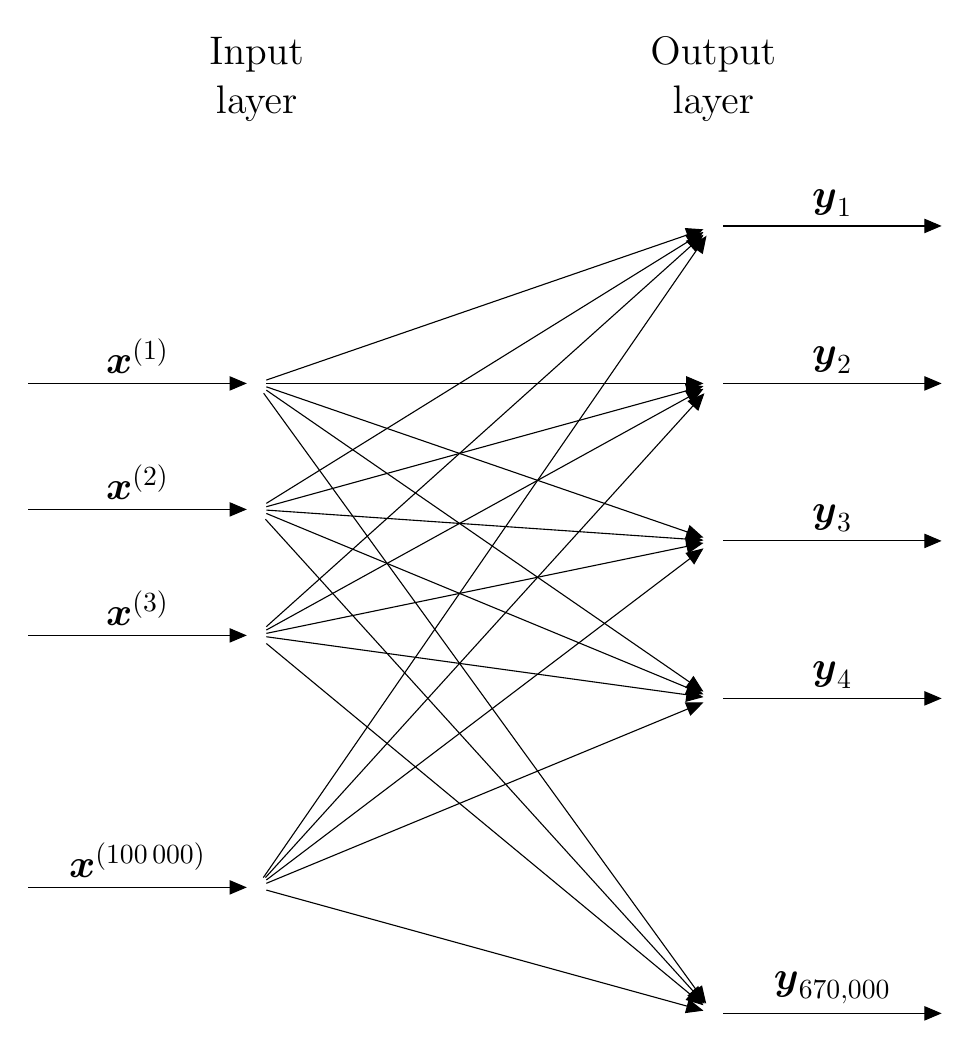
\begin{tikzpicture}[x=2.9cm, y=1.6cm, >=stealth, font=\Large]

\foreach \m/\l [count=\y] in {1,2,3,missing,4}
  \node [every neuron/.try, neuron \m/.try] (input-\m) at (0,2.5-\y) {};

\foreach \m [count=\y] in {1,2,3,4,missing,5}
  \node [every neuron/.try, neuron \m/.try ] (hidden-\m) at (2,4.0-\y*1.25) {};



%\foreach \m [count=\y] in {1,missing,2}
%  \node [every neuron/.try, neuron \m/.try ] (output-\m) at (4,1.5-\y) {};

\foreach \l [count=\i] in {1,2,3,100\,000}
  \draw [style={<-,>=triangle 45}] (input-\i) -- ++(-1,0)
    node [above, midway] {$\vec{x}^{(\l)}$};


%\foreach \l [count=\i] in {1,2}
%  \draw [->] (hidden-\i) -- ++(1,0)
%    node [above, midway] {$O_\l$};
    
    \draw [style={->,>=triangle 45}]  (hidden-1) -- ++(1,0)
    node [above, midway] {$\vec{y}_1$};
    
    \draw [style={->,>=triangle 45}]  (hidden-2) -- ++(1,0)
    node [above, midway] {$\vec{y}_{2}$};
    
    \draw [style={->,>=triangle 45}]  (hidden-3) -- ++(1,0)
    node [above, midway] {$\vec{y}_{3}$};
    
    \draw [style={->,>=triangle 45}]  (hidden-4) -- ++(1,0)
    node [above, midway] {$\vec{y}_{4}$};
    
    \draw [style={->,>=triangle 45}]  (hidden-5) -- ++(1,0)
    node [above, midway] {$\vec{y}_{670,000}$};
    
%\foreach \l [count=\i] in {1}
%  \node [above] at (hidden-1.north) {$O_1$};
%	\node [above] at (hidden-2.north) {$O_{670\,000}$};
	
  
%\foreach \l [count=\i] in {1,2}
%  \draw [->] (hidden-\i) -- ++(1,0)
%    node [above, midway] {$O_\l$};

\foreach \i in {1,...,4}
  \foreach \j in {1,...,5}
    \draw [style={->,>=triangle 45}] (input-\i) -- (hidden-\j);

    
%    \foreach \i in {1,...,3}
%  \foreach \j in {1,...,2}
%    \draw [style={->,>=triangle 45}] (input-\i) -- (hidden-\j)
%    node [above, midway] {$\textbf{W}_{(\i,\j)}$};

%    \draw [style={->,>=triangle 45}] (input-1) -- (hidden-1)
%    node [above, midway] {$\textbf{W}_{(1,1)}$};
%    
%    \draw [style={->,>=triangle 45}] (input-2) -- (hidden-1)
%    node [above, midway] {$\textbf{W}_{(2,1)}$};
%    
%    \draw [style={->,>=triangle 45}] (input-3) -- (hidden-1)
%    node [above, midway] {$\textbf{W}_{(3,1)}$};
%    
%    \draw [style={->,>=triangle 45}] (input-4) -- (hidden-1)
%    node [below, near start] {$\textbf{W}_{(51033,1)}$};
    
%    \draw [style={->,>=triangle 45}] (input-1) -- (hidden-2)
%    node [above, midway] {$\textbf{W}_{(1,2)}$};
    
%    \draw [style={->,>=triangle 45}] (input-1) -- (hidden-1)
%    node [above, midway] {$\textbf{W}_{(1,1)}$};
%    
%    \draw [style={->,>=triangle 45}] (input-1) -- (hidden-1)
%    node [above, midway] {$\textbf{W}_{(1,1)}$};  

%\foreach \i in {1,...,2}
%  \foreach \j in {1,...,2}
%    \draw [->] (hidden-\i) -- (output-\j);

\foreach \l [count=\x from 0] in {Input, Output}
  \node [align=center, above] at (\x*2,3.5) {\l \\ layer};
 

\end{tikzpicture}}\pause
%\column{0.45\columnwidth}
%\begin{itemize}
%\vspace{-0.10in}
%\item Label embedding 

%\end{itemize}
\begin{center}
\begin{huge}
\input{deep}
\end{huge}
\end{center}
%\end{columns}
\begin{itemize}
	\item Mapping input to output via embedding layer
	\item Nonlinear alternative to $A\vec{x} = VU \vec{x}$
\end{itemize}
}


\begin{frame}{Low-rank approximation in Setting A}

Factorize the matrix $Y$ instead of the parameter matrix $A$: 
\begin{center}
\includegraphics[width=11cm]{Figures/matrixcompletion2}
\end{center}
$$Y \qquad = \qquad  U \qquad \times \qquad V \qquad $$

\end{frame}

\begin{frame}{Low-rank approximation in Setting A}
{Overview of algorithms}

\begin{itemize}
\item Nuclear norm minimizationan\footnote{Candes and Recht, Exact low-rank matrix completion via convex optimization. Foundations
of Computational Mathematics 2008}
\item Gaussian processes\footnote{Lawrence and Urtasun, Non-linear matrix factorization with Gaussian processes, ICML 2009}
\item Probabilistic methods\footnote{Shan and Banerjee, Generalized probabilistic matrix factorizations for collaborative
filtering, ICDM 2010} 
\item Spectral regularization\footnote{Mazumder et al., Spectral regularization algorithms for learning large incomplete matrices., JMLR 2010} 
\item Non-negative matrix factorization\footnote{Gaujoux and Seoighe, A flexible R package for nonnegative matrix factorization.
BMC bioinformatics 2010}
\item Alternating least-squares minimization\footnote{Jain et al., Low-rank matrix completion using alternating minimization, ACM Symposium on Theory of Computing 2013}
\end{itemize}

\end{frame}

\begin{frame}{Matrix factorization with side information for Setting A}

\begin{center}
\includegraphics[scale=0.3]{pics/settingA}
\end{center}
\begin{itemize}
\item Construct \alert{implicit} features $(\vec{x}^I,\vec{t}^I)$ for users and items with matrix factorization methods
\item Exploit \alert{explicit} features $(\vec{x}^E,\vec{t}^E)$ (a.k.a. side information)
\item Concatenate: 
$$\vec{x}^C = (\vec{x}^I,\vec{x}^E), \qquad \vec{t}^C = (\vec{t}^I,\vec{t}^E)$$
\item Apply methods that we have seen before\footnote{Menon and Elkan, A log-linear model with latent features for dyadic prediction, ICDM 2010}\footnote{Volkovs and Zemel, Collaborative filtering with 17 parameters, NIPS 2012}: 
\end{itemize}
\begin{equation*}
\label{eq:pairwise}
f(\vec{x}^C,\vec{t}^C) = \vec{w}^T \big(\phi(\vec{x}^C) \otimes \psi(\vec{t}^C)\big)    
\end{equation*}
\vspace{-0.2cm}
\end{frame}

%\begin{frame}{Hybrid matrix factorization for Setting A}
%
%Basilico and Hofmann, 2004;
%Abernethy et al, 2008; Adams et al, 2010; Fang and Si, 2011; Zhou et al, 2011a; Menon and
%Elkan, 2011; Zhou et al, 2012b).
%
%\end{frame}

%\begin{frame}
%
%\begin{center}
%\includegraphics[scale=0.5]{Figures/interaction}
%\end{center}
%\begin{exampleblock}{Question}
%In which situations are relation and representation construction models capable of outperforming independent models w.r.t.\ predictive performance in Setting B? 
%\begin{itemize}
%\item Always
%\item When $n$ is sufficiently large
%\item When $m$ is sufficiently large
%\item When the targets are sufficiently correlated
%\end{itemize}
%\end{exampleblock}
%\end{frame}

%\begin{frame}{When is it useful to construct target representations?}
%\begin{center}
%Does not work well in extreme multi-label classification\footnote{Babbar and Sch\"olkopf, DISMEC: Distributed Sparse Machines for Extreme Multi-label classification, WSDM 2017}:
%
%\includegraphics[scale=0.3]{Figures/dismec} 
%\end{center}
%\end{frame}
%
%\begin{frame}{When is it useful to construct target representations?}{SVD interpretation}
%\begin{center}
%Representation of instance (or feature) \hspace{1cm} Representation of target
%\includegraphics[scale=0.5]{Figures/svd} 
%\end{center}
%\vspace{-0.3cm}
%$$p \times m \qquad \quad \qquad p \times p \qquad \qquad \qquad p \times m \qquad \qquad m \times m$$
%\vspace{-0.3cm}
%\begin{itemize}
%\item $\sigma_1,\sigma_2,...$: singular values of $A$
%\item Rank of $A$ = number of non-zero \alert{singular values} \pause 
%\item \alert{High rank} when a lot of singular values differ from zero
%\item \alert{Low rank} when a lot of singular values are zero
%\item Singular values \alert{give insight} in what can be gained
%\end{itemize}
%\end{frame}







%\begin{frame}{Can we improve on independently-learned models?}
 %\center
%\vspace{-0.5cm}
   %\includegraphics[width=\textwidth]{Figures/results1}
   %
%\end{frame}


%\begin{frame}{Some take-home messages about two-step KRR}
%
%\begin{itemize}
%\item Important to distinguish different learning settings in the general framework of multi-target prediction \pause 
%\item Two-step KRR is applicable to Settings A, B, C and D \pause 
%\item It is very easy to implement \pause 
%\item It is a universal approximator \pause 
%\item It is identical to Kronecker kernel ridge regression with a specific pairwise kernel \pause 
%\item It has two separate regularization parameters: one for instances and one for tasks \pause 
%\item It allows for interesting computational tricks
%\begin{itemize}
%\item `free' tuning for the hyperparameters \pause 
%\item `free' LOOCV \alert{for all four settings}! \pause 
%\item closed-form solution for updating with mini-batches
%\end{itemize} 
%\end{itemize}
%
%\end{frame}





\section{Conclusions}

\begin{frame}{Conclusions}

\begin{itemize}
\item Multi-target prediction is an active field of research that connects different types of machine learning problems
\item In the corresponding subfields of machine learning, problems have typically been solved in isolation, without establishing connections between methods
\item When analyzing MTP methods, it is important to understand several concepts, such as the influence of loss functions, and the availability and absence of side knowledge
\end{itemize}

\begin{center}
{\bf Corresponding paper: \\
Waegeman et al. \\ Multi-Target Prediction: \\ A Unifying View on Problems and Methods \\
Data Mining and Knowledge Discovery, 2019.}

\end{center}

\end{frame}

%\begin{frame}
%\frametitle{Many thanks to...}
%\begin{center}
%Michiel Stock, Tapio Pahikkala, Antti Airola, Bernard De Baets,  Krzysztof Dembczynski, Eyke H{\"u}llermeier and Weiwei Cheng for collaborating on this topic!
%
%\vskip18pt
%%\begin{center}
%\begin{minipage}[c]{.8\textwidth}
%\begin{center}
%
%\includegraphics[height=1.5cm]{pics/ms.jpg}
%\hskip0.5cm
%\includegraphics[height=1.5cm]{pics/tp.jpg}
%\hskip0.5cm
%\includegraphics[height=1.5cm]{pics/aa.jpg}
%\hskip0.5cm
%\includegraphics[height=1.5cm]{pics/bdb.jpg}
%\hskip0.5cm \\
%\vspace{1cm}
%\includegraphics[height=1.5cm]{pics/kd.jpg}
%\hskip1cm
%\includegraphics[height=1.5cm]{pics/eh.jpg}
%\hskip1cm
%\includegraphics[height=1.5cm]{pics/wc.jpg}
%\end{center}
%\end{minipage}
%\end{center}
%\end{frame}

%\begin{frame}{Selected references}
%\begin{itemize}
%\item T Pahikkala, M Stock, A Airola, T Aittokallio, B De Baets, W Waegeman A two-step learning approach for solving full and almost full cold start problems in dyadic prediction, ECML/PKDD 2014, 517-532 2014
%\item T. Pahikkala, A. Airola, T. Salakoski, M. Stock, B. De Baets, W. Waegeman, Efficient least-squares algorithms for conditional ranking on relational data, Machine Learning 93, p321-356, 2013
%\item M. Stock, T. Pahikkala, A. Airola, B. De Baets, W. Waegeman, Efficient Pairwise Learning Using Kernel Ridge Regression: an Exact Two-Step Method (Arxiv-preprint)
%\item W. Waegeman, K. Dembczynski, E. H\"ullermeier, A taxonomic review of multi-target prediction methods, in preparation
%\end{itemize}
%\end{frame}
%
%\bibliographystyle{plain}
%\nobibliography{references} 

\end{document}
